%%%%%%%%%%%%%%%%%%%%%%%%%%%%%%%%%%%%%%%%%
% Beamer Presentation
% LaTeX Template
% Version 1.0 (10/11/12)
%
% This template has been downloaded from:
% http://www.LaTeXTemplates.com
%
% License:
% CC BY-NC-SA 3.0 (http://creativecommons.org/licenses/by-nc-sa/3.0/)
%
%%%%%%%%%%%%%%%%%%%%%%%%%%%%%%%%%%%%%%%%%

%----------------------------------------------------------------------------------------
%	PACKAGES AND THEMES
%----------------------------------------------------------------------------------------

\documentclass{beamer}

\mode<presentation> {

% The Beamer class comes with a number of default slide themes
% which change the colors and layouts of slides. Below this is a list
% of all the themes, uncomment each in turn to see what they look like.

%\usetheme{default}
%\usetheme{AnnArbor}
%\usetheme{Antibes}
%\usetheme{Bergen}
%\usetheme{Berkeley}
%\usetheme{Berlin}
%\usetheme{Boadilla}
%\usetheme{CambridgeUS}
%\usetheme{Copenhagen}
%\usetheme{Darmstadt}
%\usetheme{Dresden}
%\usetheme{Frankfurt}
%\usetheme{Goettingen}
%\usetheme{Hannover}
%\usetheme{Ilmenau}
%\usetheme{JuanLesPins}
%\usetheme{Luebeck}
\usetheme{Madrid}
%\usetheme{Malmoe}
%\usetheme{Marburg}
%\usetheme{Montpellier}
%\usetheme{PaloAlto}
%\usetheme{Pittsburgh}
%\usetheme{Rochester}
%\usetheme{Singapore}
%\usetheme{Szeged}
%\usetheme{Warsaw}

% As well as themes, the Beamer class has a number of color themes
% for any slide theme. Uncomment each of these in turn to see how it
% changes the colors of your current slide theme.

%\usecolortheme{albatross}
%\usecolortheme{beaver}
%\usecolortheme{beetle}
%\usecolortheme{crane}
%\usecolortheme{dolphin}
%\usecolortheme{dove}
%\usecolortheme{fly}
%\usecolortheme{lily}
%\usecolortheme{orchid}
%\usecolortheme{rose}
%\usecolortheme{seagull}
%\usecolortheme{seahorse}
%\usecolortheme{whale}
%\usecolortheme{wolverine}

%\setbeamertemplate{footline} % To remove the footer line in all slides uncomment this line
%\setbeamertemplate{footline}[page number] % To replace the footer line in all slides with a simple slide count uncomment this line

%\setbeamertemplate{navigation symbols}{} % To remove the navigation symbols from the bottom of all slides uncomment this line
}

\usepackage{graphicx} % Allows including images
\usepackage{booktabs} % Allows the use of \toprule, \midrule and \bottomrule in tables
\usepackage{esint}

%----------------------------------------------------------------------------------------
%	TITLE PAGE
%----------------------------------------------------------------------------------------

\title[Non-Convex shape Collision Detection]{Efficient Probabilistic Collision Detection for Non-Convex Shapes} % The short title appears at the bottom of every slide, the full title is only on the title page

\author{Rong Yuyang} % Your name
\institute[UCDavis] % Your institution as it will appear on the bottom of every slide, may be shorthand to save space
{
University of California, Davis \\ % Your institution for the title page
\medskip
\textit{PtrRong@ucdavis.edu} % Your email address
}
\date{\today} % Date, can be changed to a custom date

\begin{document}

\begin{frame}
	\titlepage % Print the title page as the first slide
\end{frame}

\begin{frame}
	\frametitle{Overview} % Table of contents slide, comment this block out to remove it
	\tableofcontents % Throughout your presentation, if you choose to use \section{} and \subsection{} commands, these will automatically be printed on this slide as an overview of your presentation
\end{frame}

%----------------------------------------------------------------------------------------
%	PRESENTATION SLIDES
%----------------------------------------------------------------------------------------

%------------------------------------------------
\section{Motivation} % Sections can be created in order to organize your presentation into discrete blocks, all sections and subsections are automatically printed in the table of contents as an overview of the talk
%------------------------------------------------

%\subsection{Subsection Example} % A subsection can be created just before a set of slides with a common theme to further break down your presentation into chunks

\begin{frame}
	\frametitle{Motivation}
	\begin{itemize}
		\item Path(Motion) planning.
		\item Computational bottleneck, one by one comparasion is not feasiable memory-wise and time-wise.
		\item Difficult to represent(noisy observation).
	\end{itemize}
	\begin{figure}
		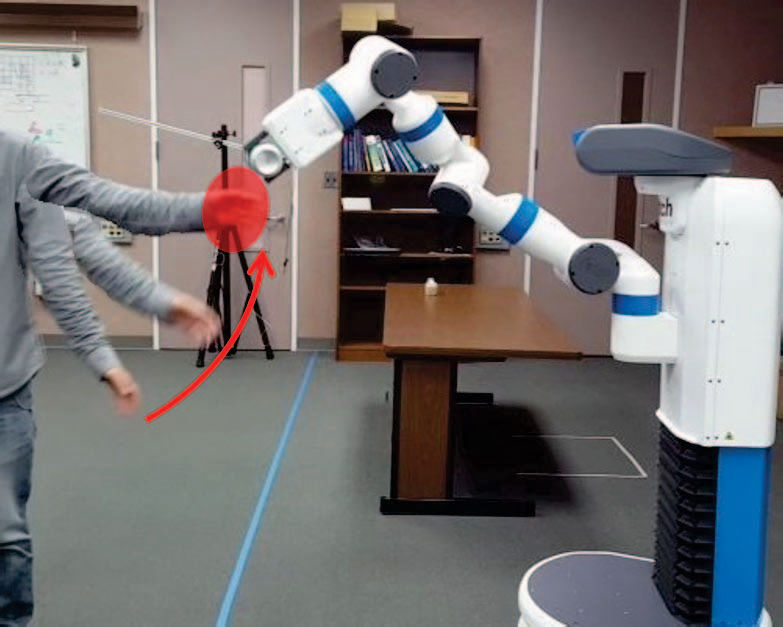
\includegraphics[width=5cm]{imgs/PS.png}
		\caption{Will they collide?}
	\end{figure}
\end{frame}

%------------------------------------------------

%------------------------------------------------
\section{Problem Statement} % Sections can be created in order to organize your presentation into discrete blocks, all sections and subsections are automatically printed in the table of contents as an overview of the talk
%------------------------------------------------

%\subsection{Subsection Example} % A subsection can be created just before a set of slides with a common theme to further break down your presentation into chunks

\begin{frame}
	\frametitle{Problem Statement}
	Given set:$A, B$(confined by meshes),
	want to know whether: 
	$$A \cap B = \emptyset$$
	True / False ?
	\textbf{Probability}!
	\\
	\textbf{Gaussian Distribution} to A required:
	$$\epsilon \sim \mathcal{N}(0, \Sigma)$$
	$$A + \epsilon := \{a+\epsilon | a \in A\}$$
	$$V := (A+\epsilon) \cap B$$
	Find: 
	$$P(V \neq \emptyset) = \iiint_Vp(\mathbf{x},0,\mathbf{\Sigma})d\,\mathbf{x}$$
\end{frame}

%------------------------------------------------
\section{Approach} % Sections can be created in order to organize your presentation into discrete blocks, all sections and subsections are automatically printed in the table of contents as an overview of the talk
%------------------------------------------------

%------------------------------------------------
%\begin{frame}
%\frametitle{Convex shape}
%	$A$ is a convex set $\Leftrightarrow$ \\ $\forall a, b \in A$, 
%	$\forall s\geq 0, t \geq 0, s+t=1$, s.t. $sa+tb \in A$
%	\begin{figure}\label{Convex}
%		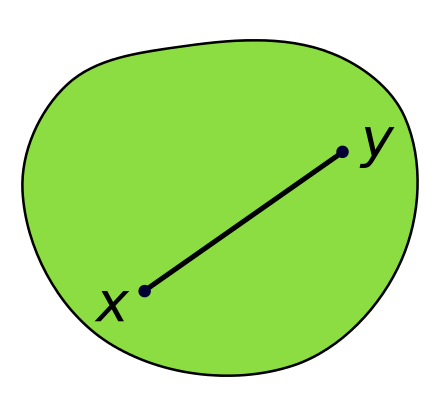
\includegraphics[width=4cm]{imgs/ConvexShape.png}
%		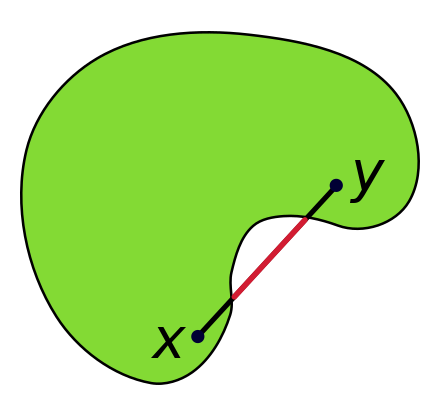
\includegraphics[width=4cm]{imgs/Non-ConvexShape.png}
%		\caption{The left hand side is a convex set while the right hand side is not.}
%	\end{figure}
%\end{frame}

%------------------------------------------------
\begin{frame}
	\frametitle{Probability on convex shape}
	\begin{itemize}
		\item Normalize Gaussian Distribution: $A' = (\Sigma^{-\frac{1}{2}})A$, $B' = (\Sigma^{-\frac{1}{2}})B$.
		\item Calculate Minkowski Sum: $V' = A' + B'$. Property: For two convex hull, the result is a convex space. $O(|V'|)$
		\item Divergence Theorem: Integration over $V'$ transformed to $S'$, where $S'$ is the surface of $V'$
		\item Mesh representation approximation \& Upper Bound approximation:
		      $$\oiint_{S'}\mathbf{F}\cdot\mathbf{n_s}\,dS \leq \sum_i(\max_{j = 1,2,3}\mathbf{F}(S_{ij})\cdot\mathbf{n}_i)S_{\Delta S_{i1}S_{i2}S_{i3}}$$
		      $$P_{real} \leq P_{calculated}$$
	\end{itemize}
\end{frame}

%------------------------------------------------
\begin{frame}
	\frametitle{Probability on non-convex shape: approach}
	\begin{itemize}
		\item Take non-convex shape apart.
		\item Form a bounding volume hierarchies(BVHs)
		\item Many methods for this available: spheres, AABBs, OBBs, etc)
	\end{itemize}
	\begin{figure}
		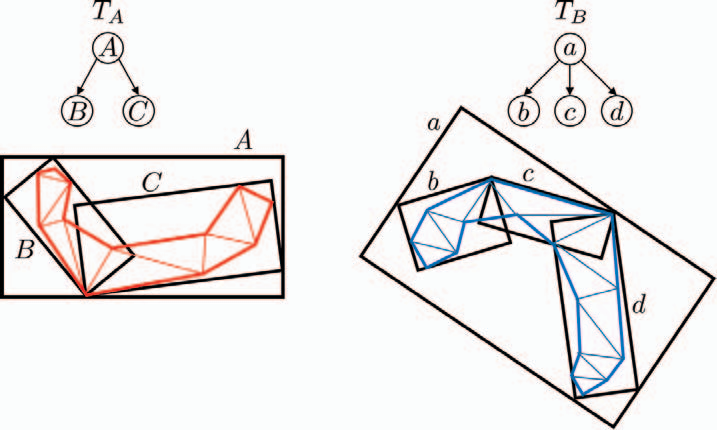
\includegraphics[width=5cm]{imgs/a.png}
		\caption{An example using OBBs to form BVH.}
	\end{figure}
\end{frame}

%------------------------------------------------
\begin{frame}
	\frametitle{Probability on non-convex shape: calculation}
	\begin{itemize}
		\item Set confidence level$\delta_{CD} < 1$(normally $\delta_{CD} > 0.9$).
		\item Compare $P_{calculated}$ with $1-\delta_{CD}$
		\item Be more specific if $P_{calculated} > 1-\delta_{CD}$
	\end{itemize}
	%	\begin{figure}	
	%		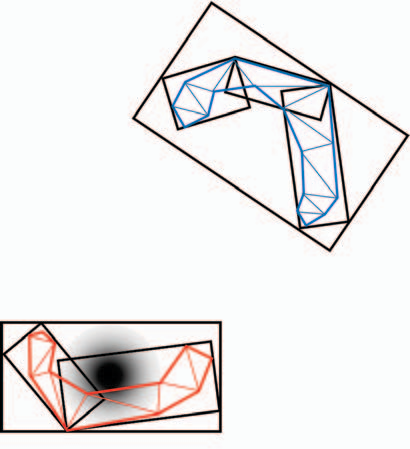
\includegraphics[width=2cm]{imgs/b.png}
	%		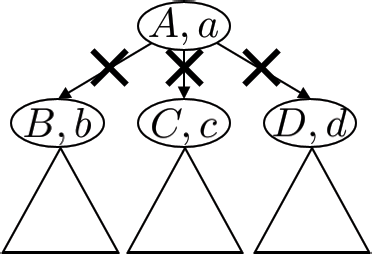
\includegraphics[width=2cm]{imgs/c.png}
	%		\caption{Boxes so far away that no more detection is required.}
	%	\end{figure}
	%	\begin{figure}	
	%		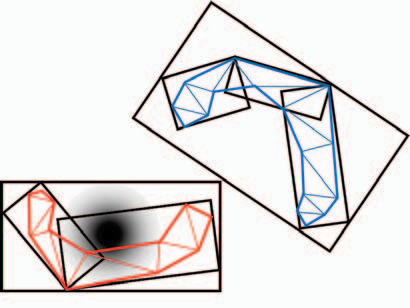
\includegraphics[width=2cm]{imgs/d.png}
	%		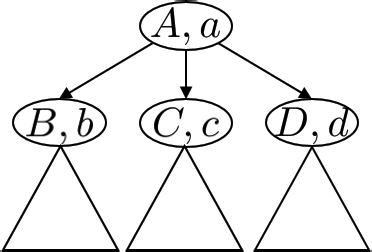
\includegraphics[width=2cm]{imgs/e.png}
	%		\caption{We are not sure about the bounding box so we do the further checking.}
	%	\end{figure}
\end{frame}

%------------------------------------------------
\begin{frame}
	\frametitle{Probability on non-convex shape: example}
	\begin{figure}	
		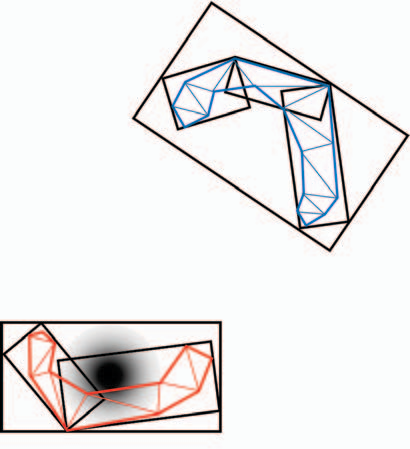
\includegraphics[width=2.5cm]{imgs/b.png}
		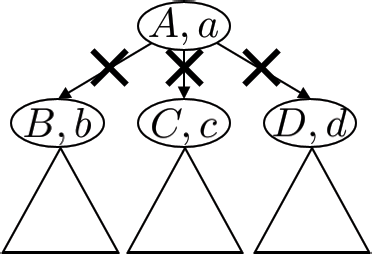
\includegraphics[width=2.5cm]{imgs/c.png}
		\caption{Boxes so far away that no more detection is required.}
	\end{figure}
	\begin{figure}	
		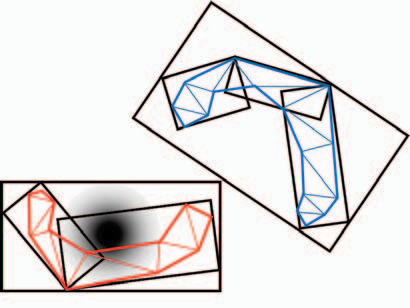
\includegraphics[width=2.5cm]{imgs/d.png}
		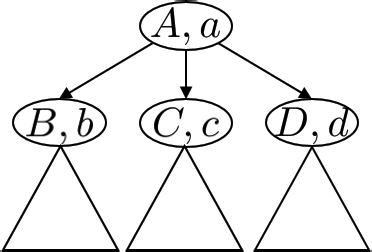
\includegraphics[width=2.5cm]{imgs/e.png}
		\caption{We are not sure about the bounding box so we do the further checking.}
	\end{figure}
\end{frame}

%------------------------------------------------
\section{Experiments}
%------------------------------------------------
%------------------------------------------------
\begin{frame}
	\frametitle{Experiments}
	\begin{figure}	
		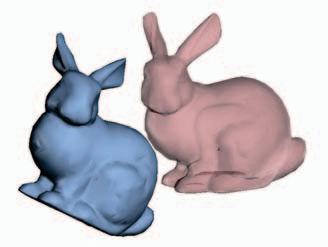
\includegraphics[width=2.5cm]{imgs/Benchmark1.png}
		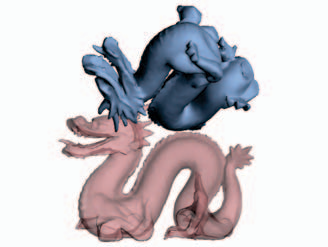
\includegraphics[width=2.5cm]{imgs/Benchmark2.png}
		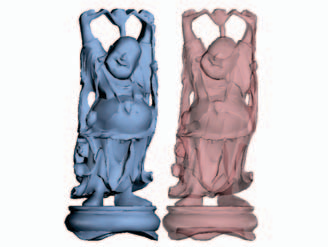
\includegraphics[width=2.5cm]{imgs/Benchmark3.png}
		\caption{Benchmark \#1(5,110 meshes), \#2(10,000 meshes), \#3(10,000 meshes)}
	\end{figure}
	\begin{figure}	
		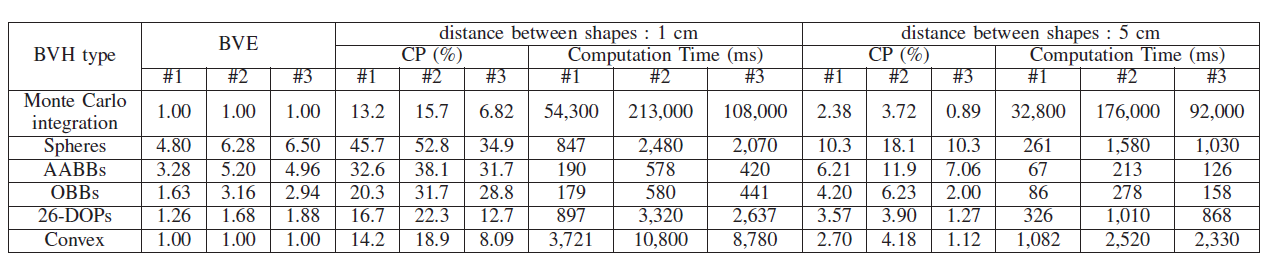
\includegraphics[width=12cm]{imgs/Table.png}
		\caption{Results}
	\end{figure}
\end{frame}



%------------------------------------------------
\section{Conclusion}
%------------------------------------------------

\begin{frame}
	\frametitle{Conclusion}
	\begin{itemize}
		\item Probabilistic collision detection for general shapes.
		\item Fast and reliable
		\item Drawback: only translation collision, rotation not considered.
	\end{itemize}
\end{frame}

%------------------------------------------------
\end{document} \grid
